\chapter{Backend Explained} \label{Backend Explained}

In this chapter I will document the contents of the backend project and challenges met along the development process.

\section{Project Configuration}

\subsection{Parent Project}

\noindent The backend main project is a multi-module Maven project. 
In a multi-module Maven project, the parent POM (Project Object Model) serves as the primary configuration file that defines common settings, dependencies, and plugins for all the modules within the project. It helps to centralize and manage configurations that are shared across multiple modules, promoting consistency and reducing redundancy. Additionally, the parent POM can define build profiles, repositories, and other project-wide settings that are inherited by all child modules.
\\\\
\noindent In the \textbf{pom.xml} from \hl{/backend/pom.xml} (Figure \ref{fig:figure2}), essential metadata settings are defined, including groupId, artifactId, version, modules, and packaging. Additionally, a parent is specified, namely \hl{spring-boot-starter-parent} from org.springframework.boot, which provides default configurations and dependencies for Spring Boot applications. Right after, global variables are utilized to specify the Java version (17), set the project encoding as UTF-8, and define other reusable values, such as library versions. Following this, \textbf{two profiles}, "dev" and "prod", are declared to facilitate switching between running modes. These profiles determine the file configurations used in the Spring Boot applications. Next, \textbf{dependencies} and \textbf{dependencyManagement} settings are specified. The \hl{spring-boot-starter-web} from org.springframework.boot is added as a dependency to all modules, pulling in web development-related dependencies like an embedded Tomcat server and data binding. DependencyManagement, a setting specific to the parent pom.xml, provides general configurations for potential dependencies without directly including them. It primarily serves to globally specify library versions, eliminating the need to specify versions in each file when imported in modules. Similarly, within the \textbf{build} setting, \textbf{plugins} and \textbf{pluginManagement} are utilized. The \hl{maven-compiler-plugin} is imported in all modules for packaging applications into JARs. In pluginManagement, configuration settings for the mapping library \textbf{MapStruct} are specified, and \hl{spring-boot-maven-plugin} is instructed to exclude Project Lombok's code. These configurations can be overridden in child modules if necessary.

\begin{figure}[h]
    \centering
    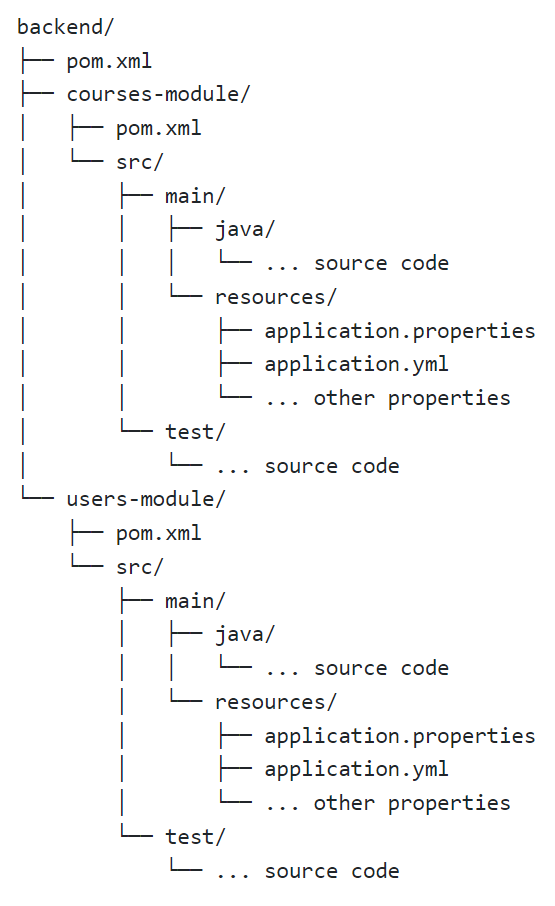
\includegraphics[scale=0.7]{images/backend-folder-structure.png}
    \caption{Backend - Folder structure}
    \label{fig:figure2}
\end{figure}

\subsection{Users Module Project} \label{Users Module Project}

\noindent In the \textbf{pom.xml} from \hl{/backend/users-module/pom.xml} (Figure \ref{fig:figure2}), alongside standard metadata, the dependencies utilized in this module are declared. These dependencies include \textbf{mapstruct}, \textbf{mapstruct-processor}, \textbf{lombok}, \textbf{spring-boot-starter-data-jpa}, \textbf{hibernate-core}, \textbf{hibernate-hikaricp}, \textbf{postgresql}, \textbf{spring-boot-starter-test}, \textbf{junit-jupiter-api}, \textbf{h2}, \textbf{jjwt-api}, \textbf{jjwt-impl}, \textbf{jjwt-jackson}, and \textbf{caffeine}. Further details about their usage will be provided in subsequent sections.
\\\\\newpage
\noindent In the \textbf{resources folder} from \hl{/backend/users-module/src/main/resources} (Figure \ref{fig:figure2}) are located configuration and property files for Spring Boot.
\\\\
\noindent A \textbf{banner.txt} file that is displayed right in the beginning of the application. It contains written in big text the name of the module, as well as the module's version and spring boot's version. This information can be useful for monitoring and letting you know if you are running with outdated software.
\\\\
\noindent When it comes to application settings, Spring Boot automatically recognizes two types of files: \textbf{application.yml} and \textbf{application.properties}. The distinction lies in their usage, as application.properties supports only string values, while application.yml is better suited for handling complex values and nested properties. In the users module, both types of files are used. This approach allows for a separation between common and generic settings in application.yml, while custom properties are managed in application.properties.
\\\\
\noindent In the configuration from inside \textbf{application.yml}, the \textbf{server.port} property specifies the port used to start the Embedded Tomcat Server. It's crucial to assign a unique port to avoid conflicts with other applications. The \textbf{spring.profiles.active} property determines the active profiles for the application, obtained through the \textbf{@activatedProperties@} placeholder, replaced by Maven based on the \textbf{<activatedProperties>} tag.
\\\\
\noindent The section for configuring the HikariCP \cite{hikaricp} connection pool includes properties such as \textbf{connection-timeout}, \textbf{idle-timeout}, \textbf{max-lifetime}, \textbf{minimum-idle}, \textbf{maximum-pool-size}, and \textbf{pool-name}. These properties define parameters like maximum wait time for a connection, maximum idle time, maximum lifetime of a connection, minimum number of idle connections, maximum pool size, and the pool name, respectively.
\\\\
\noindent The properties \textbf{ddl-auto} and \textbf{show-sql} relate to Hibernate and JPA. ddl-auto specifies how Hibernate handles database schema updates based on entity mappings, set here to "update" to allow for automatic schema updates based on their corresponding Java entity. show-sql controls whether queries executed by Hibernate are logged, aiding in debugging database operations and helping with performance, allowing you to see if manual query optimization is required.
\\\\
\noindent Finally, \textbf{server.error.include-message} determines whether error messages are included in error responses sent by the server. In this case, error messages are included, aiding in debugging and error handling for the REST API backend. By default, these messages are hidden to prevent leakage of private code logic information, but that is handled via custom error processors in this web platform.
\\\\
\noindent Based on selected profile, Spring Boot can use conditional files. For example, for an active profile x and an inactive profile y, \mbox{\textbf{application-x.properties}} will be loaded but \mbox{\textbf{application-y.properties}} will not.
\\\\
\noindent In the \textbf{application-dev.properties} file of the users module, several settings are configured to manage database connectivity, H2 console access, JPA behavior, data seeding, and logging levels. The \textbf{spring.datasource.url} setting specifies the URL used to connect to the database, with the example provided connecting to an H2 in-memory database named DesignOOP-UsersDB. Credentials for database authentication are defined with \textbf{spring.datasource.username} and \textbf{spring.datasource.password}, set to sa and an empty string, respectively, for running an instance of the module in development mode. The JDBC driver class name is specified with \textbf{spring.datasource.driver-class-name}, set to org.h2.Driver for the H2 database. The \textbf{spring.h2.console.enabled} setting determines whether the H2 console is enabled, allowing browser-based interaction with the database when set to true. Additionally, the Hibernate dialect for JPA is configured with spring.jpa.database-platform, set to org.hibernate.dialect.H2Dialect for compatibility with H2. Data seeding, the process of populating the database with initial data, is controlled by \textbf{app.data.seeding.enabled}, set to true to enable seeding. This feature is needed for testing purposes, as H2 is used as an in-memory database, that resets its content on each restart. Finally, logging levels for specific packages or classes are configured with logging.level, with debug-level logging enabled for Spring MVC method invocation (\textbf{org.springframework.web.servlet.mvc.method.annotation}) and Spring Security-related classes (\textbf{org.springframework.security}).
\\\\
\noindent In the \textbf{application-prod.properties} file of the users module, database connectivity settings are configured to connect to a PostgreSQL database. The \textbf{datasource.url}, \textbf{datasource.username}, and \textbf{datasource.password} settings specify the JDBC URL, username, and password for accessing the database, respectively. These values are placeholders (\$\{POSTGRES\_URL\}, \$\{POSTGRES\_USERNAME\}, \$\{POSTGRES\_PASSWORD\}) that are replaced with actual values stored in environment variables or property files. The database type is set to PostgreSQL via \textbf{jpa.database}, and the JDBC driver class name is specified with \textbf{datasource.driver-class-name}, set to org.postgresql.Driver for PostgreSQL databases. Additional Hibernate properties are configured with \textbf{jpa.properties}, including \textbf{hibernate.format\_sql} set to true to format SQL queries for readability, and hibernate.dialect set to \textbf{PostgreSQLDialect} to specify the dialect for PostgreSQL databases.
\\\\
\noindent The \textbf{application.properties} file contains custom settings regarding JWT settings.

\subsection{Courses Module Project}

\noindent In the \textbf{pom.xml} from \hl{/backend/courses-module/pom.xml} (Figure \ref{fig:figure2}) are declared the dependencies for the course module. They include \textbf{mapstruct}, \textbf{mapstruct-processor}, \textbf{spring-boot-starter-data-mongodb}, \textbf{spring-boot-starter-security}, \textbf{spring-boot-starter-oauth2-resource-server}, \textbf{spring-security-oauth2}, \textbf{lombok}. Further details about their usage will appear in subsequent sections.
\\\\
\noindent Configuration and property files for Spring Boot are located in the \textbf{resources folder} from \hl{/backend/courses-module/src/main/resources} (Figure \ref{fig:figure2}). The purpose of the files present in this folder (\textbf{banner.txt}, \textbf{application.yml}, \textbf{application.properties}, \textbf{application-[profile].properties}) is already described in the beginning of the \ref{Users Module Project} subsection.
\\\\
\noindent In the configuration provided, the \textbf{server.port} property specifies the port for the Embedded Tomcat Server, ensuring it operates on a unique port to avoid conflicts with other applications. The \textbf{spring.profiles.active} property determines the active profiles for the application, dynamically assigned based on Maven's \textbf{<activatedProperties>} tag, allowing for flexible configuration.
\\\\
\noindent The section for configuring the MongoDB database includes properties such as \textbf{auto-index-creation}, \textbf{authentication-database}, \textbf{username}, \textbf{password}, \textbf{database}, \textbf{host}, and \textbf{port}. These properties define parameters such as auto-index creation, authentication details, database credentials, and connection details, ensuring seamless integration with the MongoDB database. Some of the previously mentioned fields use placeholders, that will be replaced by environmental variables (\$\{mongodb\_username\}, \$\{mongodb\_password\}, \$\{mongodb\_database\}, \$\{mongodb\_host\}, \$\{mongodb\_port\}).
\\\\
\noindent The \textbf{server.error.include-message} property determines whether error messages are included in error responses sent by the server. Enabling this property aids in debugging and error handling for the REST API backend. By default, these messages are hidden to prevent leakage of private code logic information, but custom error processors handle them within this web platform.
\\\\
\noindent When the development profile is active, extra debugging information is enabled via the \textbf{logging.level.org.springframework.web.servlet.mvc.method.annotation} and the
\textbf{logging.level.org.springframework.security} properties, which are set to "DEBUG" inside the \textbf{applications-dev.properties} file.

\section{Folder structure of a module}

To ensure code maintainability, all modules in this web platform representing Spring Boot applications follow the folder structure shown in Figure \ref{fig:figure3}.

\begin{figure}[h]
    \centering
    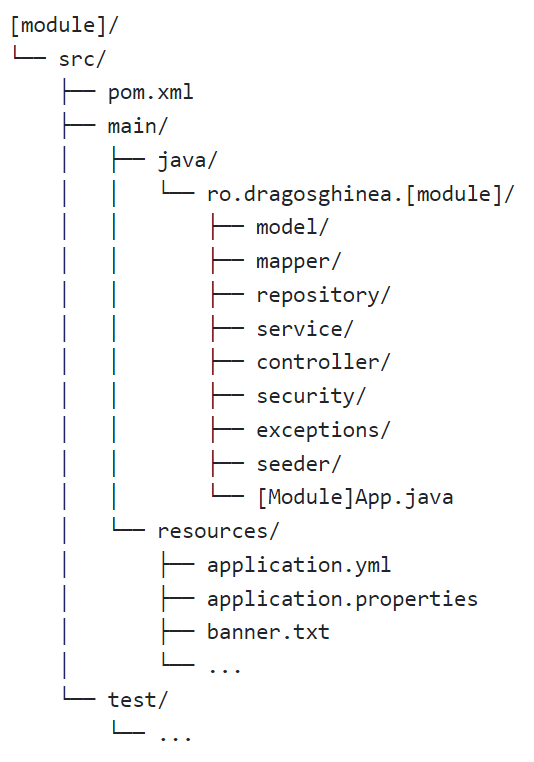
\includegraphics[scale=0.7]{images/module-folder-structure.png}
    \caption{Module - Folder structure}
    \label{fig:figure3}
\end{figure}

\noindent This folder structure is a template for the modules, but if required, more packages could be created besides the ones specified in \hl{ro.dragosghinea.[module]}. In fact, from the ones mentioned in Figure \ref{fig:figure3}, only \textbf{model}, \textbf{repository}, \textbf{service}, \textbf{controller} are crucial, as they are the base of the repository-controller-service pattern that I try to enforce in Spring Boot modules. More details regarding each package present in the main folder of the module are described in the following sections.

\section{Repositories}

In the repository-service-controller pattern, the role of the repository classes is to communicate with the database, executing transactions. As a separation of concerns and structured hierarchy, repositories are supposed to only be accessed by the services. For repositories, important are the \textbf{repository} and \textbf{model} packages from Figure \ref{fig:figure3}.
\\\\
\noindent Inside \textbf{repository} are defined repository interfaces, that contain methods for interacting with the database. These interfaces have automatic implementations by Spring Data, which are influenced by method definitions and, if necessary, custom queries specified using the \textbf{@Query} annotation. Notably, complex queries can be automatically generated based on method names. For instance, the method signature \verb|List<Person>| \verb|findDistinctPeopleByLastnameOrFirstname(String lastname, String firstname);| produces a query that precisely fulfills its name's intent. For further insights into this behavior, refer to \cite{spring-data-repositories}. Additionally, Spring Data can accommodate different return types, such as returning \textbf{null} for a find method with a return type of \textbf{Entity}, or an \textbf{Optional<Entity>} returning an empty value.
\\\\
\noindent In the \textbf{model} package, you'll find classes designated as entities, which are utilized by Spring Data to interact with the database. Additionally, this package contains special objects known as data transfer objects (DTOs), which facilitate communication with higher layers such as services and controllers. Data transfer objects serve a crucial role in decoupling, as their usage detaches information from the database. Direct manipulation of entities can inadvertently trigger unwanted database updates, making DTOs a preferred choice for communication between layers or anywhere outside the database interaction domain.

\subsection{Users Module}

\subsubsection{Model}

\noindent The users module uses Spring Data JPA as the primary interface, implemented via Hibernate. The entities of the module are created via \textbf{@Entity} and \textbf{@Table} annotations. The @Entity annotation marks the class as a JPA entity. The @Table annotation allows customization of the entity, allowing the addition of foreign keys and changing the name of the table used for the entity (by default, the class name is also the table name).

\begin{figure}[h]
    \centering
    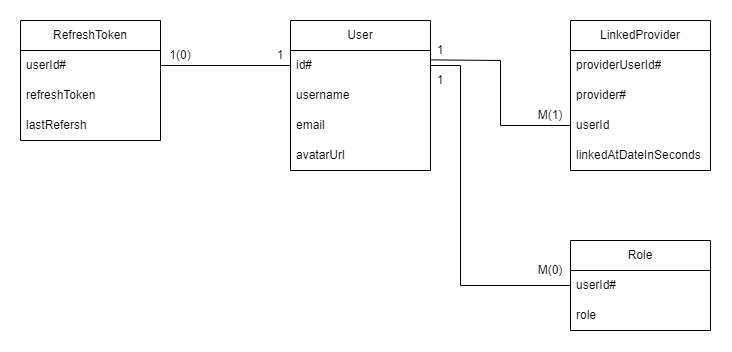
\includegraphics[scale=0.6]{images/users-schema.png}
    \caption{Users Database Schema}
    \label{fig:figure4}
\end{figure}

\newpage
\noindent In the users module, there are corresponding classes for the entities represented in Figure \ref{fig:figure4}. Classes annotated with \textbf{@Entity} are RefreshToken, User, and LinkedProvider. The Role entity is not an actual class, as the annotation \textbf{@ElementCollection} is used inside the User entity. This annotation automatically takes an iterable collection and maps it to a separate table.
\\\\
The \textbf{@Table} annotation is used for two purposes in this module. Firstly, to rename the User entity to "User\_", as the name without an underscore seems to be reserved by the database's internal mechanics. This is done via \textbf{@Table(name="USER\_")}. The second purpose is declaring unique key constraints, done via the {@Table(uniqueConstraints = {...}} in the LinkedProvider entity. Besides the composite primary key, the LinkedProvider should have the unique composite key \textbf{(provider, userId)}, ensuring a user doesn't have two external providers of the same type linked. Code wise, the unique constraint is defined via \textbf{@UniqueConstraint(name="OneProviderPerUser", columnNames = \{"user\_id", "provider"\})}.
\\\\
\noindent In the model classes, entity relationships are defined using fields with special annotations. The relationship between the LinkedProvider and User entities is established through two fields, although only one is necessary for the relationship to be recognized. In the LinkedProvider class, the \textbf{\textit{private User user;}} field is annotated with \textbf{@ManyToOne}. This annotation includes a parameter (fetch=FetchType.LAZY), instructing Hibernate to retrieve this field from the database only when it's accessed via a call. Similarly, the User class denotes the relationship with the \textbf{@OneToMany} annotation and the \textbf{\textit{List<LinkedProvider> linkedProviders;}} field. The \textbf{cascade = CascadeType.ALL} parameter ensures that all linked providers are deleted if the corresponding user is deleted, allowing for cascading events. Incorporating both the userId and user field within the LinkedProvider presented some challenges, which were addressed by adding two annotations. The userId field is annotated with @Column(user\_id), while the user field uses @JoinColumn(name = "user\_id", referencedColumnName = "id", insertable = false, updatable = false). The @JoinColumn annotation enables the entity to exist without automatically persisting modifications to the database made through the user field. A similar relationship is established between the User and RefreshToken entities.
\\\\
\noindent In addition to the entities, corresponding DTOs are created to facilitate communication in upper layers such as services and controllers. Alongside these entity-specific DTOs, there are also additional DTOs that don't directly correspond to specific entities but contain information utilized for certain requests.

\subsubsection{Repository}

\noindent In the users module, repositories are interfaces that extend the \textbf{JpaRepository<\\EntityClass, EntityIdClass>} type. This JpaRepository, a part of Spring Data, inherits functionality from CrudRepository, which handles CRUD operations like findById, save, and deleteById, as well as from PagingAndSortingRepository, which adds methods for pagination and sorting. With repositories defined for nearly all entities shown in Figure \ref{fig:figure4}, automatic and custom-generated queries are utilized. An automatic query example is \textit{LinkedProvider findByProviderUserIdAndProvider(String providerUserId, ProviderType provider)}, which performs the action described by its method name. Custom queries are also employed in the users module, such as the need to eagerly load a lazy field without making two trips to the database, as demonstrated by the annotation \textit{@Query("SELECT rt FROM RefreshToken rt JOIN FETCH rt.user WHERE rt.userId = :userId")}.

\subsection{Courses Module}

\subsubsection{Model}

\noindent The courses module uses Spring Data MongoDB, where entities are annotated with \textbf{@Document}. MongoDB was chosen for its suitability to handle dynamic elements like courses, which may evolve over time without a fixed design. For instance, if additional metadata needs to be added to course objects in the future, MongoDB seamlessly accommodates these changes without requiring database refactorings, as its document-based structure automatically adapts to new fields. The recursive nature of the component tree in courses would have posed challenges with a relational database, given its lack of structured definition. Since courses are manipulated as JSONs on the frontend and no complex queries benefiting from relational databases are anticipated on the server side, MongoDB emerged as the optimal choice, offering storage in BSON format closely aligned with JSON.
\\\\
\noindent The courses module's most complex operation is the \textbf{full-text search feature}, aimed at retrieving relevant courses based on user input. Initially, specialized database systems like Elasticsearch were considered for their scalability and indexing capabilities. However, configuring support for both MongoDB and Elasticsearch proved challenging and excessive for the current use case. While Elasticsearch remains a viable option for future scalability needs, the chosen approach for the current platform is to utilize MongoDB's built-in text search feature.
\\\\
\noindent To enable this feature, the Course entity defines multiple text indexes using \textbf{@TextIndexed} with varying weights, which are later merged into a single full-text search index applied to the database. It's essential to ensure that \textbf{auto-index-creation} is set to true in Spring Boot's properties to facilitate index creation.
\\\\
\noindent The \textbf{full-text search} functionality matches against multiple properties with different weights to calculate a relevancy score. These properties, ranked in order of importance from highest to lowest, include title, tags, subtitle, description, and components content. For specifying the weights for each property, the weight parameter is utilized in the @TextIndexed annotation. The text score is returned inside the entity via a float field, annotated with @TextScore.

\subsubsection{Repository}

\noindent In the courses repository, the Spring Data \textbf{MongoRepository<EntityClass, EntityIdClass>} interface is extended along with a custom CourseSearchRepository interface. Similar to JpaRepository used in the users module, MongoRepository provides common CRUD and pagination methods.
\\\\
\noindent The custom CourseSearchRepository interface exposes a new method: \textit{Page<Course> search(String query, int pageNumber, int pageSize, boolean fetchWithoutComponents)}. This method conditionally excludes the \textbf{components} field from the returned values based on the fetchWithoutComponents parameter. This optimization reduces payload size since only metadata, not content, is essential for presenting search results to users.
\\\\
\noindent The CourseSearchRepository interface is implemented through a custom implementation, \textbf{CourseSearchRepositoryImpl}, which utilizes MongoTemplate to execute the search query. In this implementation, the query string is matched as a case-insensitive phrase with ignored diacritics. The resulting List, wrapped in a Page format, is sorted by the text score. Spring automatically detects and uses the custom implementation of CourseSearchRepository. The custom implementation was done with the help of the following online resource: \cite{mongodb-custom-repositories}.

\section{Services}

Services, responsible for executing algorithms, manipulating data, and interfacing with repositories, constitute the business logic layer in the web platform's modules. They are mainly called by controllers or other services, while they, in turn, call repositories. Ideally, they should all reside within the \textbf{service} package, as indicated in Figure \ref{fig:figure3}, with the exception of security-related services, which are placed separately in the security package.
\\\\
\noindent Mappers, essential for converting objects between different types, are predominantly utilized in the backend for mapping DTOs to entities and vice versa. The web platform uses \textbf{MapStruct} to automate the generation of mappers. This library identifies interfaces annotated with \textbf{@Mapper} and compiles implementations during build time. However, a challenge arises due to caching issues, where changes to mapped classes may not trigger the generation of new implementations. Consequently, runtime errors may occur during mapping attempts. To avoid this issue, it's advisable to perform a Maven clean operation before compiling, or at least upon encountering mapper-related errors.

\subsection{Users Module}

\noindent In the users module, the primary focus lies on authentication. Several services handle authentication against various linked providers like Discord or GitHub. Additionally, there's a general authentication service responsible for invoking the appropriate service based on the input type. Apart from these, there are two services dedicated to CRUD operations: one for user CRUD and another for refresh tokens CRUD. Further details on refresh tokens can be found in the security section.
\\\\
\noindent Within this module, service methods declare their return type and parameters using DTOs, while internally operating with entities. Consequently, each service requires both a repository instance and a mapper instance. To address this, a compositional approach is adopted. Fields for the necessary instances are defined within the services and initialized via a parameterized constructor. Lombok facilitates this process with its \textbf{@RequiredArgsConstructor} annotation, which automatically generates a constructor with parameters for all final fields within the annotated class. Spring Boot handles the instantiation of these services through \textbf{dependency injection}. By recognizing the dependencies of a constructor, Spring Boot constructs and retains instances of those dependencies, injecting them when creating instances of the parameterized service.

\subsection{Courses Module}

\noindent In the courses module, the primary focus revolves around resource management. Consequently, the service within this module is responsible for handling CRUD operations related to courses. Unlike JPA, the MongoDB integration of Spring Data does not automatically persist changes and is not as tightly coupled to the database session. Therefore, the decision was made not to create a DTO for the course object. However, in the context of DTOs, a class was created specifically to facilitate communication of page data to the controller. This class, named PageDto, is essentially a mapping of Spring's Page class, but with select fields renamed and additional fields added as needed.

\section{Controllers}

Controllers serve as the entry point for a REST API, exposing routes that can be accessed via HTTP requests. They orchestrate the business logic defined in services, maintaining a separation of concerns by communicating only with services and not directly with repositories. In this web platform, controller classes are located in the \textbf{controller} package (Figure \ref{fig:figure3}), identified by the \textbf{@RestController} annotation.
\\\\
\noindent Routes are defined using annotations, such as \textbf{@RequestMapping}, which sets the base route for all methods within the class, and method-specific annotations like \textbf{@GetMapping}, \textbf{@PostMapping}, \textbf{@DeleteMapping}, and \textbf{@PutMapping} to define the HTTP methods for individual routes. These annotations can also have a value parameter to extend the route specified by the controller class.
\\\\
\noindent Data validation is automatically handled by Spring Boot, rejecting requests with parameters that don't match the method's object parameters. Additional validation, like password length or email format, can be implemented separately. Annotations like \textbf{@RequestHeader}, \textbf{@RequestParam}, \textbf{@PathVariable}, and \textbf{@RequestBody} are used to extract data from different parts of the request, such as headers, query parameters, dynamic path segments, and the request body, respectively. There are other specialized annotations available for specific request elements as well.
\\\\
\noindent For \textbf{exception handling}, three approaches are employed, inspired by \cite{baeldung-spring-exceptions}. \textbf{The first approach} involves handling exceptions at the controller layer. If an error occurs within a controller method, a \textbf{ResponseStatusException} is thrown to indicate the specific HTTP status code and error message. \textbf{The second approach} utilizes a global controller exception handler defined using \textbf{@ControllerAdvice}. This class can intercept and handle errors thrown within controllers, allowing for centralized exception handling and customization of the response. \textbf{The third approach} involves annotating exceptions thrown by services with \textbf{@ResponseStatus}. This annotation specifies the HTTP status code to be returned when the exception is encountered, allowing the default error resolver to handle it appropriately.

\begin{lstlisting}[style=json, frame=single, caption={error response format}, label={lst:listing1}]
{
    "timestamp": date string,
    "status": HttpStatusCode,
    "error": HttpStatusError,
    "message": error string,
    "path": route string
}
\end{lstlisting}

\noindent In listing \ref{lst:listing1}, the error format follows a standard commonly used in Spring Boot applications. It includes several key fields: \textbf{timestamp} indicates the exact time when the error occurred, formatted as an ISO 8601 string (YYYY-MM-DDTHH:MM:SS.sss±hh:mm); \textbf{status} represents the HTTP status code of the response to the request; \textbf{error} denotes the associated error category corresponding to the error status (e.g., "Not found" for error status 404); \textbf{message} provides a human-readable error message; \textbf{path} specifies the route at which the error was thrown.

\subsection{Users Module}

In this subsection, the entry points of the users module are explained, resembling a REST API documentation. This module consists of two controllers with distinct purposes. One controller manages authentication and token generation, handling routes starting with \textbf{/v1/auth}, while the other allows user profile customization and manages routes starting with \textbf{/v1/users}.
\\\\
\noindent The \textcolor{olive}{GET} \textbf{/v1/users/me} route fetches the user details for the currently logged-in user. An unauthorized request response is sent if this route is accessed without an authenticated user.
\\\\
\noindent The \textcolor{cyan}{PATCH} \textbf{/v1/users/me} route updates user details. It receives a body with the fields of the user that need an update. It can be a single field or multiple.
\\\\
\noindent The \textcolor{orange}{POST} \textbf{/v1/auth/login} route handles user login, expecting a clientRegistrationId and an accessToken in the request body. The clientRegistrationId represents the OAuth2 provider (e.g., Discord or GitHub), while the accessToken is a valid OAuth2 access token. Upon validation, user information is extracted and a new access token with a refresh token is returned.
\\\\
\noindent The \textcolor{orange}{POST} \textbf{/v1/auth/logout} route simply logs out the currently authenticated user that executes the request.
\\\\
\noindent The \textcolor{orange}{POST} \textbf{/v1/auth/refresh} route generates a new access token based on a refresh token. The refresh token can be passed as a header (\textbf{refresh-token}) or as a parameter in the request body (\textbf{refresh\_token}). To optimize performance, a cache using the \textbf{Caffeine} library stores recently generated tokens for 3 seconds, preventing excessive token regeneration. If a cache value is returned, the response body will signal it via a message field.
\\\\
\noindent The \textcolor{orange}{POST} \textbf{/v1/auth/validate-token} route validates backend access tokens (not OAuth2 tokens generated by Discord or GitHub), returning a response status code of 200 for valid tokens and 401 for invalid ones.

\subsection{Courses Module}

In this subsection, the entry points of the courses module are explained, resembling a REST API documentation.
\\\\
\noindent The \textcolor{olive}{\textbf{GET}} \textbf{/v1/courses} route retrieves courses and accepts optional query parameters: \textbf{pageNumber} (default: 0), \textbf{pageSize} (default: 20), and \textbf{search} for filtering courses based on a phrase. Additionally, the custom request header \textbf{X-Fetch-Without-Components} can be provided to optimize payload by excluding course components when unnecessary.
\\\\
\noindent The \textcolor{orange}{\textbf{POST}} \textbf{/v1/courses} route creates a new course. It expects a request body containing all course fields except the ID, which is optional and auto-generated if absent. The newly created course is returned, containing the generated ID if one was not given.
\\\\
\noindent The \textcolor{blue}{\textbf{PUT}} \textbf{/v1/courses/\{courseId\}} route updates a course identified by \{courseId\}. It receives the updated course in the request body, with the ID remaining unchanged.
\\\\
\noindent The \textcolor{red}{\textbf{DELETE}} \textbf{/v1/courses/\{courseId\}} route deletes a course specified by \{courseId\}, without requiring additional parameters or request body.
\\\\
\noindent The \textcolor{olive}{\textbf{GET}} \textbf{/v1/courses/\{courseId\}} route fetches details of a specific course, identified by \{courseId\}. No additional parameters are considered.

\section{Security}

The security of the backend relies heavily on \textbf{Spring Security}. In the context of this web platform, there are two main types of backend modules: resource servers and authorization servers. The users module acts as the \textbf{authorization server}, responsible for generating access and refresh tokens and managing their validity. On the other hand, the courses module serves as the \textbf{resource server}, verifying all tokens using the users module.
\\\\
\noindent Security-related services and configurations are located within the security package (see Figure \ref{fig:figure3}). The primary security configuration can be found in the \textbf{SecurityConfig} class, which is annotated with both \textbf{@Configuration} and \textbf{@EnableWebSecurity}. In this configuration, CORS protection is enabled while CSRF protection is disabled.
\\\\
\noindent \textbf{CORS (Cross-Origin Resource Sharing)} protection is essential to prevent unauthorized access from other domains to resources. Although not typically recommended for public REST APIs due to potential accessibility limitations, for this web platform, access is restricted to known sources only. Therefore, the CORS configuration specifies only the frontend and other modules as allowed origins for all methods.
\\\\
\noindent \textbf{CSRF (Cross-Site Request Forgery)} is a security vulnerability that enables attackers to execute requests on behalf of authenticated users. Exploiting this vulnerability involves sending a malicious link to an authenticated user. Upon clicking, the link triggers requests using the user's session, typically retrieved from browser cookies or localStorage. Given that the REST API currently serves as an internal API only, implementing CSRF protection is deemed unnecessary. Instead, session protection is entrusted to frontend and middleware security measures.
\\\\
\noindent In managing user authentication, \textbf{JWT tokens} are employed. They offer numerous advantages, including their stateless, decentralized nature, making them self-contained and secure. Additionally, they are compact and lightweight, enhancing application performance. To seamlessly integrate JWT tokens into the backend, Spring Security's session creation policy is configured as stateless. A custom token authentication provider is utilized, which accepts authentication of type \textbf{UsernameAndPasswordAuthenticationToken}. Here, the "username" corresponds to the client provider type, while the "password" represents an OAuth2 access token. Leveraging a service that extracts user information from the linked provider and maps it to a user within the web platform, a new authentication is generated based on the retrieved user data.
\\\\
\noindent The tokens are generated by a token service, which receives a secret and two expiration times via Spring's \textbf{@Value} annotation. This service utilizes the secret to sign the tokens, while the expiration times determine the lifespan of the access and refresh tokens. Storing sensitive information within these tokens is discouraged. Therefore, for this web platform, only the email address and user roles are encoded within them.
\\\\
\noindent To convert the access token into an authentication object containing the logged-in user, a OncePerRequestFilter is implemented. This custom JwtAuthenticationFilter runs before each controller method, leveraging Spring Security's \textbf{chain of responsibility}. It facilitates the use of an authorization object injected by Spring within the controller methods.
\\\\
\noindent One of the challenges with JWT tokens is their invalidation process. Merely deleting the token from the user's browser upon logout isn't sufficient, as it might still be retained by an attacker for later use. This necessitates a trade-off between the efficiency of stateless tokens and the security of stored sessions. In this system, although access tokens aren't stored, the users module maintains the refresh tokens. This approach limits the number of active tokens per user, allowing only one refresh token with a corresponding access token to be valid at any given time. If the refresh token is invalidated, so is the access token associated with it. Refresh tokens are stored in the database with an additional field indicating the latest date they were used to generate a new access token. When a user validates their access token, the users module searches the database for the corresponding refresh token. If found, it checks the latest refresh date. If the token was generated before this latest refresh date, it's considered invalid. When no refresh token is found in the database, any access token for that user is also deemed invalid. Since the latest refresh date is updated with each refresh, this ensures that only one valid access token can exist for a user at any given time.
\\\\
\noindent On resource servers, the validation of tokens is facilitated by enabling oauth2ResourceServer in Spring Security's configuration. This resource server implementation incorporates a custom JWT decoder and an object post processor, which in turn injects a custom authentication entry point for handling failures. However, injecting this custom authentication entry point posed more challenges than expected. Initially, attempts to specify it within oauth2ResourceServer or at the httpBasic level within Spring Security's configuration proved redundant, as errors were not being caught as anticipated. The solution to this dilemma was found in utilizing withObjectPostProcessor, as elaborated in a discussion referenced here \cite{springsecurity-github-issue-failhandler}.
\\\\
\noindent Within the SecurityConfig, a custom JWT Decoder @Bean is instantiated. This decoder first parses the JWT before validating it through a custom JWTValidator. This validator performs a request to the users service to verify the JWT's validity. Parsing the JWT before validation is a deliberate step aimed at optimizing the process. By parsing first, unnecessary requests for poorly validated JWT tokens are avoided.
\\\\
\noindent Additional configuration is necessary for authorization. To extract user authorities from the JWT access token, the authorities field must be utilized. Thus, a custom \textbf{JwtAuthenticationConverter} is instantiated via @Bean to specifically handle this field. Once the user's authorities are mapped, controller annotations can be employed for authorization purposes. The \textbf{@PreAuthorize} annotation enables various checks on the authenticated user. For instance, the creation of courses is annotated with \textbf{@PreAuthorize("hasAuthority('ROLE\_COURSE\_MANAGER')")}, which permits only course managers to access this route. To enable this annotation, the \textbf{@EnableMethodSecurity} annotation must be activated in the main class of the Spring Boot application.
\\\\
\noindent The usage of custom JWT Decoder and custom JwtAuthenticationConverter for the OAuth2 Resource Server was inspired by \cite{spring-security-resource-server}.
\\\\
\noindent To enhance security concerning controller errors, a CustomErrorAttributes bean is implemented, extending \textbf{DefaultErrorAttributes}. This custom implementation serves to identify "Internal Server Error" exceptions, typically unhandled errors that expose internal logic. Upon detection, the implementation generates a SHA256 hash, replacing the error message. To access the original error message, the pair (hash, message) is logged within Spring Boot. This hash value functions as a reference ID, ensuring that the error remains private and accessible only to individuals with access to the backend's internal logic.
\\\\
\noindent To define a default admin with access to all areas within the platform, a custom Spring Boot configuration property (\textbf{default\_admin\_email}) is used. This property is injected via \textbf{@Value} in a @Configuration class named \textbf{DefaultAdmin}. When building the JWT token and specifying authorities, a check is performed to determine if the user is the default admin. If so, the user's existing roles are overwritten with the roles assigned to the default admin. Currently, since there are no negative roles like "BANNED", the admin is granted all roles. The identity of the default admin is not private information in this context, so discovering the email does not compromise the application. Furthermore, the email is declared outside the application and specified in a Spring Boot property for flexibility, rather than using a hardcoded value.

\section{Testing}

Two main approaches are used for testing the modules: unit testing and route testing via Postman.
\\\\
\noindent For unit testing, \textbf{JUnit5} \cite{junit5} is used. JUnit5 is a testing framework for Java that provides annotations for component testing. The tests created with JUnit5 are located in the \textbf{test} package shown in Figure \ref{fig:figure3}. Unit testing offers several benefits: it provides confidence that the code runs as expected if all tests pass, acts as documentation by showing the expected behavior, and speeds up development due to the automated nature of the tests, which makes running them easy and fast compared to manually setting up an environment and executing actions.
\\\\
\noindent To achieve isolation in tests, \textbf{Mockito} \cite{baeldung-mockito} is employed. Mockito is a framework that can mock the dependencies of the components being tested, ensuring that any exceptions thrown are caused by the component under test, not by external factors. For example, it allows testing the business logic of a service independently of the logic within its dependent repositories or mappers. This is achieved by hardcoding the return values of methods in the dependencies, so they provide the expected objects.
\\\\
\noindent While the tests are primarily designed as unit tests, the inclusion of the \textbf{@SpringBootTest} annotation unintentionally transforms them into integration tests. This occurs as the annotation triggers the initialization of the entire application context before running the tests. This approach is adopted to facilitate the testing of instances injected by Spring Boot.
\\\\
\noindent Tests can be run via \hl{mvn test} or by running the test class directly from the IDE. The results are displayed in the console, indicating details regarding the tests that were executed. Failed tests present a stack trace, showing the location of the failure. Before running the tests, environment variables for running the modules in test mode must be set. For this reason, the testing phase is excluded from the packaging process, and the tests must be run separately beforehand. In Figure \ref{fig:intellij-tests} is shown a successful test execution in IntelliJ IDEA for the users module. The left side of the image displays the list of tests, while the right side shows the console output during their execution.

\begin{figure}[h]
    \centering
    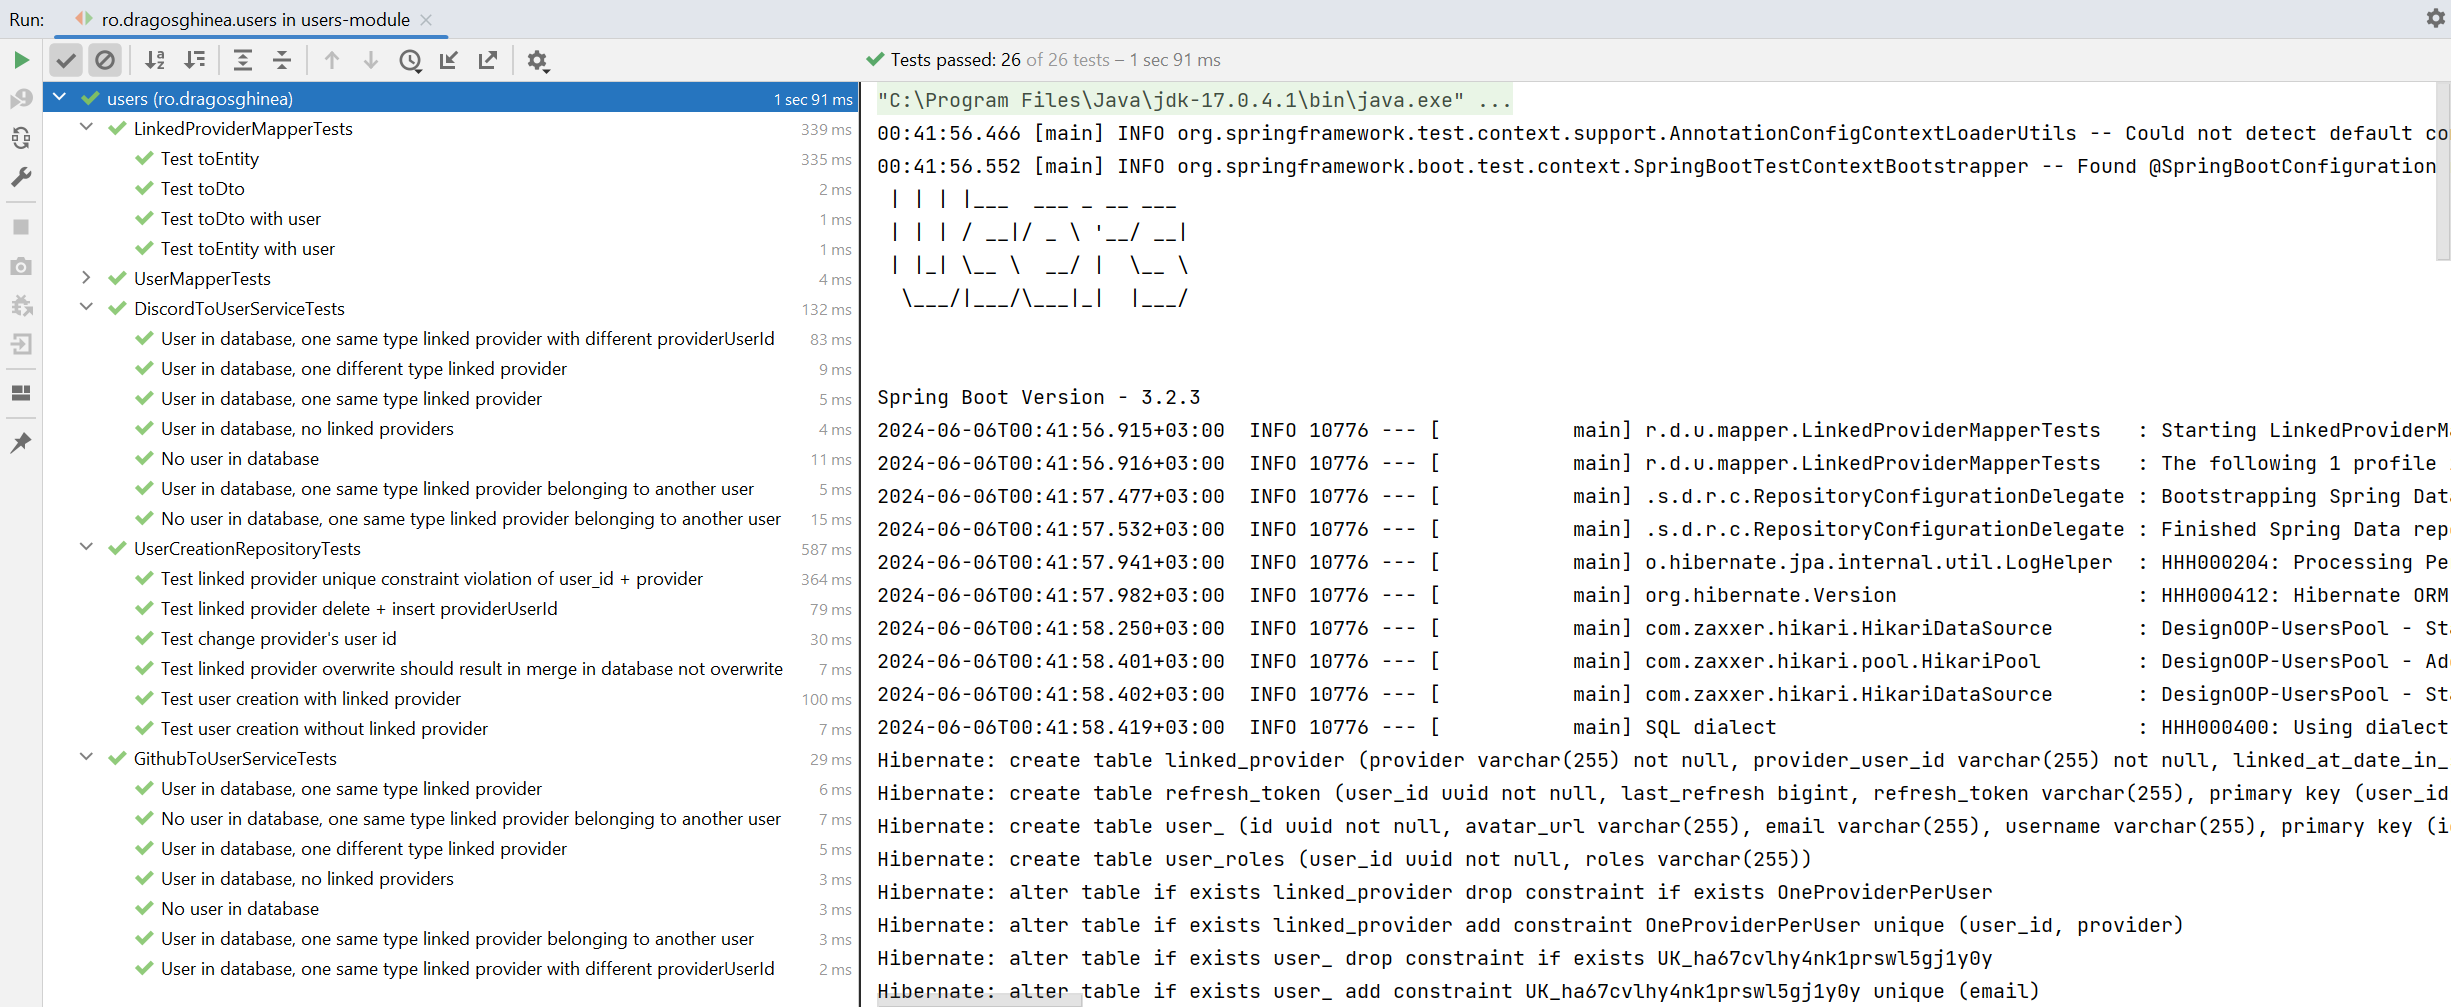
\includegraphics[trim={0 0 17cm 0},clip, width=\textwidth]{images/intellij-tests.png}
    \caption{Tests executed in IntelliJ IDEA}
    \label{fig:intellij-tests}
\end{figure}

\noindent \textbf{Postman} \cite{postman} serves as an API development tool enabling users to execute intricate requests and document them. Within this web platform, it was employed for manual route testing, involving tasks such as verifying correct request parsing, assessing response format, and inspecting backend side effects upon route access.

\begin{figure}[h]
    \centering
    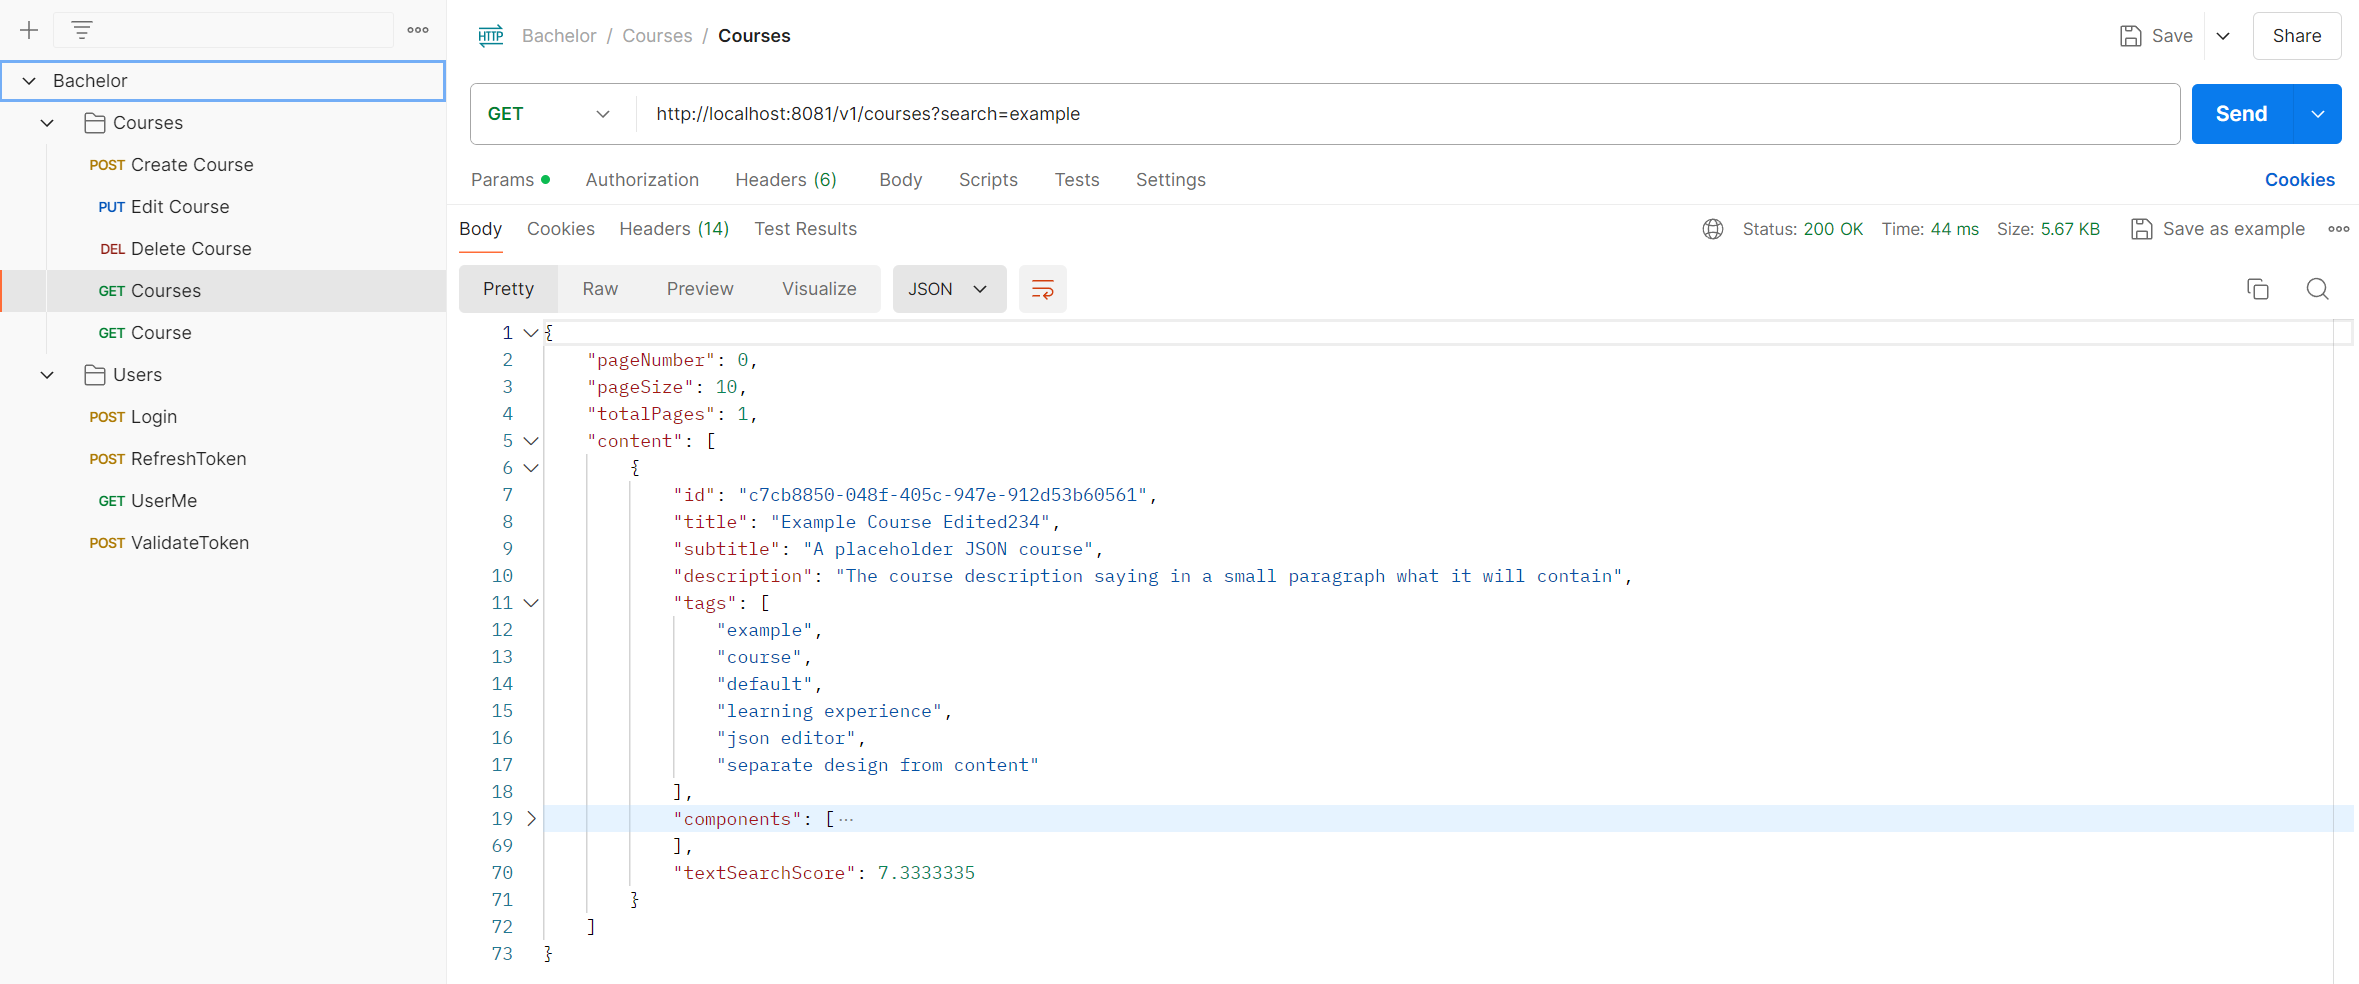
\includegraphics[trim={0 0 20cm 0},clip, width=\textwidth]{images/postman.png}
    \caption{Postman Interface}
    \label{fig:postman}
\end{figure}

\noindent In Figure \ref{fig:postman} the Postman interface is displayed, showcasing the collections and some requests used for testing the routes. The image also displays the response format for a successful GET request used to fetch the list of courses, using a search query. From the response, we can see that the courses are paginated and that each course has a text search score.
\\\\
\noindent In the future, Postman can also be used to document the API, as it provides features for adding descriptions and examples to collections and requests.